% Options for packages loaded elsewhere
\PassOptionsToPackage{unicode}{hyperref}
\PassOptionsToPackage{hyphens}{url}
\documentclass[
  11pt,
]{article}
\usepackage{xcolor}
\usepackage[margin=2.2cm]{geometry}
\usepackage{amsmath,amssymb}
\setcounter{secnumdepth}{-\maxdimen} % remove section numbering
\usepackage{iftex}
\ifPDFTeX
  \usepackage[T1]{fontenc}
  \usepackage[utf8]{inputenc}
  \usepackage{textcomp} % provide euro and other symbols
\else % if luatex or xetex
  \usepackage{unicode-math} % this also loads fontspec
  \defaultfontfeatures{Scale=MatchLowercase}
  \defaultfontfeatures[\rmfamily]{Ligatures=TeX,Scale=1}
\fi
\usepackage{lmodern}
\ifPDFTeX\else
  % xetex/luatex font selection
\fi
% Use upquote if available, for straight quotes in verbatim environments
\IfFileExists{upquote.sty}{\usepackage{upquote}}{}
\IfFileExists{microtype.sty}{% use microtype if available
  \usepackage[]{microtype}
  \UseMicrotypeSet[protrusion]{basicmath} % disable protrusion for tt fonts
}{}
\makeatletter
\@ifundefined{KOMAClassName}{% if non-KOMA class
  \IfFileExists{parskip.sty}{%
    \usepackage{parskip}
  }{% else
    \setlength{\parindent}{0pt}
    \setlength{\parskip}{6pt plus 2pt minus 1pt}}
}{% if KOMA class
  \KOMAoptions{parskip=half}}
\makeatother
\usepackage{longtable,booktabs,array}
\newcounter{none} % for unnumbered tables
\usepackage{calc} % for calculating minipage widths
% Correct order of tables after \paragraph or \subparagraph
\usepackage{etoolbox}
\makeatletter
\patchcmd\longtable{\par}{\if@noskipsec\mbox{}\fi\par}{}{}
\makeatother
% Allow footnotes in longtable head/foot
\IfFileExists{footnotehyper.sty}{\usepackage{footnotehyper}}{\usepackage{footnote}}
\makesavenoteenv{longtable}
\usepackage{graphicx}
\makeatletter
\newsavebox\pandoc@box
\newcommand*\pandocbounded[1]{% scales image to fit in text height/width
  \sbox\pandoc@box{#1}%
  \Gscale@div\@tempa{\textheight}{\dimexpr\ht\pandoc@box+\dp\pandoc@box\relax}%
  \Gscale@div\@tempb{\linewidth}{\wd\pandoc@box}%
  \ifdim\@tempb\p@<\@tempa\p@\let\@tempa\@tempb\fi% select the smaller of both
  \ifdim\@tempa\p@<\p@\scalebox{\@tempa}{\usebox\pandoc@box}%
  \else\usebox{\pandoc@box}%
  \fi%
}
% Set default figure placement to htbp
\def\fps@figure{htbp}
\makeatother
% definitions for citeproc citations
\NewDocumentCommand\citeproctext{}{}
\NewDocumentCommand\citeproc{mm}{%
  \begingroup\def\citeproctext{#2}\cite{#1}\endgroup}
\makeatletter
 % allow citations to break across lines
 \let\@cite@ofmt\@firstofone
 % avoid brackets around text for \cite:
 \def\@biblabel#1{}
 \def\@cite#1#2{{#1\if@tempswa , #2\fi}}
\makeatother
\newlength{\cslhangindent}
\setlength{\cslhangindent}{1.5em}
\newlength{\csllabelwidth}
\setlength{\csllabelwidth}{3em}
\newenvironment{CSLReferences}[2] % #1 hanging-indent, #2 entry-spacing
 {\begin{list}{}{%
  \setlength{\itemindent}{0pt}
  \setlength{\leftmargin}{0pt}
  \setlength{\parsep}{0pt}
  % turn on hanging indent if param 1 is 1
  \ifodd #1
   \setlength{\leftmargin}{\cslhangindent}
   \setlength{\itemindent}{-1\cslhangindent}
  \fi
  % set entry spacing
  \setlength{\itemsep}{#2\baselineskip}}}
 {\end{list}}
\usepackage{calc}
\newcommand{\CSLBlock}[1]{\hfill\break\parbox[t]{\linewidth}{\strut\ignorespaces#1\strut}}
\newcommand{\CSLLeftMargin}[1]{\parbox[t]{\csllabelwidth}{\strut#1\strut}}
\newcommand{\CSLRightInline}[1]{\parbox[t]{\linewidth - \csllabelwidth}{\strut#1\strut}}
\newcommand{\CSLIndent}[1]{\hspace{\cslhangindent}#1}
\setlength{\emergencystretch}{3em} % prevent overfull lines
\providecommand{\tightlist}{%
  \setlength{\itemsep}{0pt}\setlength{\parskip}{0pt}}
\usepackage{bookmark}
\IfFileExists{xurl.sty}{\usepackage{xurl}}{} % add URL line breaks if available
\urlstyle{same}
\hypersetup{
  pdftitle={Eleven winters{,} ten Diwalis: separating weather{,} farm fires and fireworks in India's PM2.5{,} 2016--2026},
  pdfauthor={Krishnav Agarwal · School of Computer Science, Vellore Institute of Technology (VIT), Vellore, India · agarwalkrishnav34@gmail.com},
  pdfkeywords={PM2.5, Diwali, crop residue burning, weather
normalisation, VIIRS, data censoring, exploratory data analysis, India},
  hidelinks,
  pdfcreator={LaTeX via pandoc}}

\title{Eleven winters, ten Diwalis: separating weather, farm fires and
fireworks in India's PM2.5, 2016--2026}
\author{Krishnav Agarwal · School of Computer Science, Vellore Institute
of Technology (VIT), Vellore, India · agarwalkrishnav34@gmail.com}
\date{Preprint · 13 October 2026 ·
https://github.com/krishnav1412/eleven-winters}

\begin{document}
\maketitle
\begin{abstract}
Delhi's winter air is usually blamed on three things that arrive
together: stagnant weather, smoke from paddy-residue fires in Punjab and
Haryana, and Diwali fireworks. We separate them in an exploratory
analysis of hourly data from 105 monitoring sites in 39 Indian cities
(2016--2026), NASA VIIRS fire detections and ERA5 weather.
Gradient-boosted models remove the effect of weather and, for Delhi, of
farm-fire smoke carried by the wind; what remains on Diwali night is the
festival's own contribution. Diwali's lunar date moved between 19
October and 14 November over the decade, and Delhi's firecracker rules
changed four times, which lets us compare like with like. Three findings
stand out. First, the reference monitor at the US Embassy stops
reporting during the worst hours of Diwali night: 52\% of late-night
Diwali hours are missing, against 4\% on ordinary autumn nights, so
averages built on it understate the festival. Second, using the
less-censored CPCB network median, Diwali night adds 127--392 µg/m³
above the weather-and-fire baseline in every year observed, 6 of 7
nights beyond the 99th percentile of ordinary nights, and years with a
full ban were not lower than years with green crackers. Third, VIIRS
detections in Punjab and Haryana fell 94\% between 2021 and 2025, but
the share caught by the 1:30 am pass rose from 0.2\% to 4.7\%, and in
2025 each detected fire went with a roughly tenfold larger rise in
Delhi's weather-adjusted PM2.5, though with wide uncertainty. Both are
consistent with burning that has moved out of the satellite's daytime
view. We publish a locked, checksummed forecast for Diwali 2026 and
release all code, derived data and an interactive companion site.
\end{abstract}

\section{Introduction}\label{introduction}

Every October and November, PM2.5 in Delhi climbs to many times the
Indian 24-hour standard of 60 µg/m³. Three explanations dominate public
debate. The first is meteorology: as the monsoon withdraws, the boundary
layer becomes shallow, winds slacken and pollution builds up. The second
is the burning of paddy residue in Punjab and Haryana, whose smoke
north-westerly winds carry towards Delhi. The third is Diwali, which in
most years falls inside the same weeks and brings a night of fireworks.

Because the three arrive together, a high reading in early November
cannot be pinned on any one of them by looking at it. Earlier work has
addressed parts of the problem. Weather-normalisation with machine
learning (\citeproc{ref-grange2018}{Grange et al. 2018}) has been
applied to Delhi (\citeproc{ref-verma2025}{Verma et al. 2025}) and to
India's National Clean Air Programme cities
(\citeproc{ref-hei_ncap}{Health Effects Institute 2025}). The best-known
causal estimate of the Diwali effect used an event-study design for
2013--2017 but did not separate firecracker smoke from crop smoke
(\citeproc{ref-ghei2018}{Ghei and Sane 2018}). On the farm-fire side,
recent studies report that burning in Punjab now happens later in the
afternoon, after the polar-orbiting satellites have passed
(\citeproc{ref-nasaeo2025}{NASA Earth Observatory 2025};
\citeproc{ref-iforest2025}{{iFOREST} 2025};
\citeproc{ref-biswal2025}{Biswal et al. 2025}), and that Delhi's PM2.5
has become only weakly coupled to official fire counts
(\citeproc{ref-mangaraj2025}{{Mangaraj et al.} 2025}).

This study uses three things that change from year to year to pull the
causes apart (Fig. 1). Diwali follows the lunar calendar, so its date
moves across the burning season: in some years it comes before the main
burning, in others in the middle of it. Delhi's firecracker rules
changed from no effective restriction (2016--2017) to green crackers in
fixed hours (2018--2019), a full ban (2020--2024) and back to green
crackers in 2025 (\citeproc{ref-dh2025}{Deccan Herald 2025}). And the
timing of crop burning itself appears to have shifted.

Our contributions are:

\begin{enumerate}
\def\labelenumi{\arabic{enumi}.}
\tightlist
\item
  A weather-and-fire baseline for Delhi's hourly PM2.5, against which
  each Diwali night is compared with 211 ordinary autumn nights scored
  the same way.
\item
  Evidence that the reference monitor most often used for Delhi goes
  dark at the peak of Diwali night, and a censoring-aware way to measure
  the festival.
\item
  A satellite-internal signature of the shift in burning time: a rise in
  the share of fires caught by VIIRS's night pass, which needs no other
  satellite.
\item
  A season-by-season estimate of how strongly Delhi's PM2.5 tracks
  upwind fire detections.
\item
  A pre-registered forecast for Diwali 2026, and an open, one-command
  pipeline that rebuilds every number, figure and the companion website.
\end{enumerate}

\begin{figure}
\centering
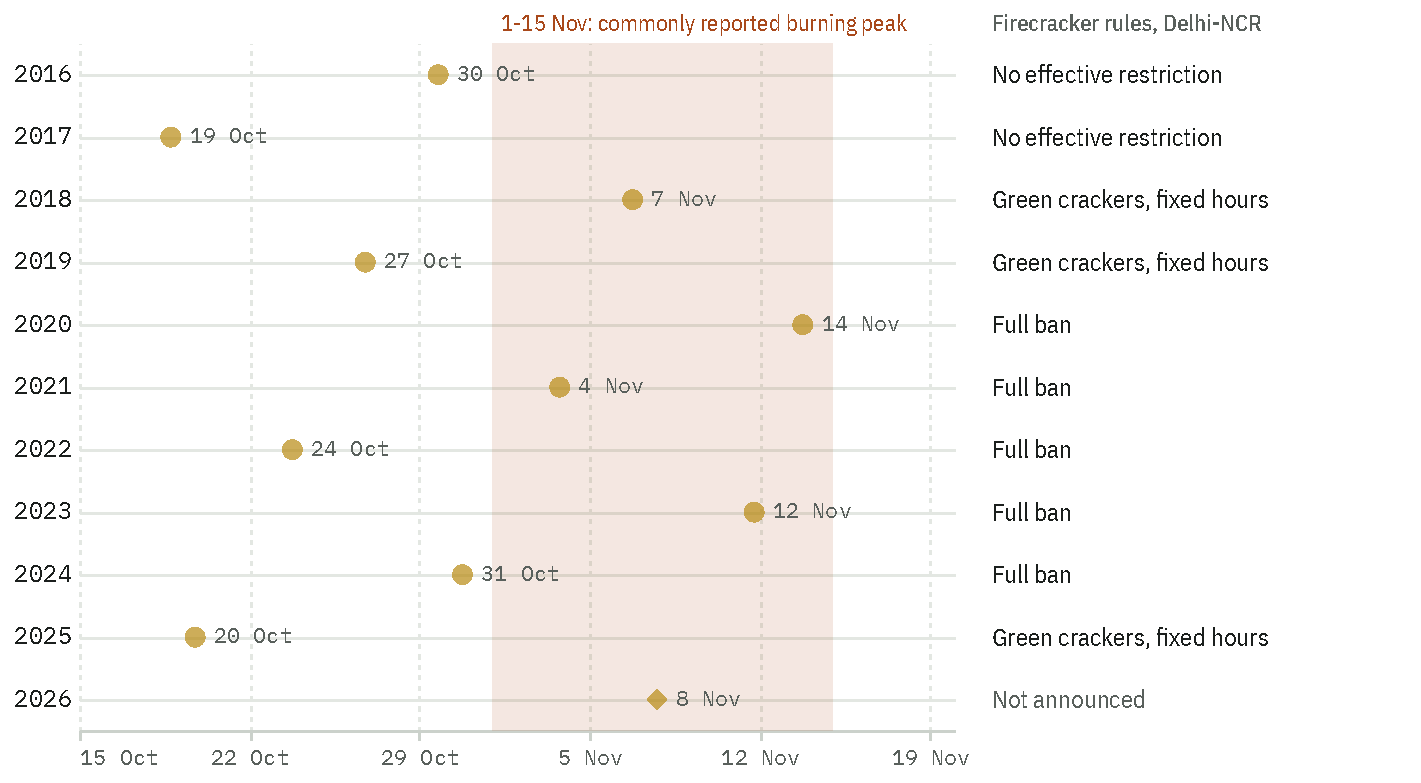
\includegraphics[width=1\linewidth,height=\textheight,keepaspectratio,alt={Diwali (Lakshmi Puja) dates, 2016--2026, and the firecracker rules in force in Delhi-NCR. The shaded band marks 1--15 November, commonly reported as the peak of paddy-residue burning.}]{figures/fig01_design.pdf}
\caption{Diwali (Lakshmi Puja) dates, 2016--2026, and the firecracker
rules in force in Delhi-NCR. The shaded band marks 1--15 November,
commonly reported as the peak of paddy-residue burning.}
\end{figure}

\section{Data}\label{data}

\subsection{Air-quality monitors}\label{air-quality-monitors}

Hourly concentrations of PM2.5, PM10, NO₂, SO₂ and CO come from the
public OpenAQ archive (\citeproc{ref-openaq}{OpenAQ 2026}), which
republishes the Central Pollution Control Board (CPCB) continuous
monitoring network and the US Department of State's embassy and
consulate monitors. We matched monitors to 39 study cities by distance
and kept the longest-running sites in each, giving 100 CPCB-network
sites and 5 US-mission sites (132 archive locations, since the same
physical monitor often appears under two identifiers after a change of
data feed). The archive timestamps mark the end of each averaging
period; we label each hour by its start.

The archive has a gap that matters for this study: CPCB-network data are
absent from late 2022 to early 2025 (Fig. 2). The US-mission monitors,
which use reference beta-attenuation instruments, run almost without
interruption, so the US Embassy in New Delhi provides the only
continuous decade-long record for Delhi.

Quality control removed 4.6\% of 2,841,635 site-hours of PM2.5: values
at or below zero or at the instrument ceiling, runs of six or more
identical readings, single-hour spikes far above both neighbours, PM2.5
above PM10, and a pattern we call a stall, in which a high reading is
repeated for one or two hours just before the record goes blank.
Multi-hour events such as Diwali nights are deliberately not removed.

\begin{figure}
\centering
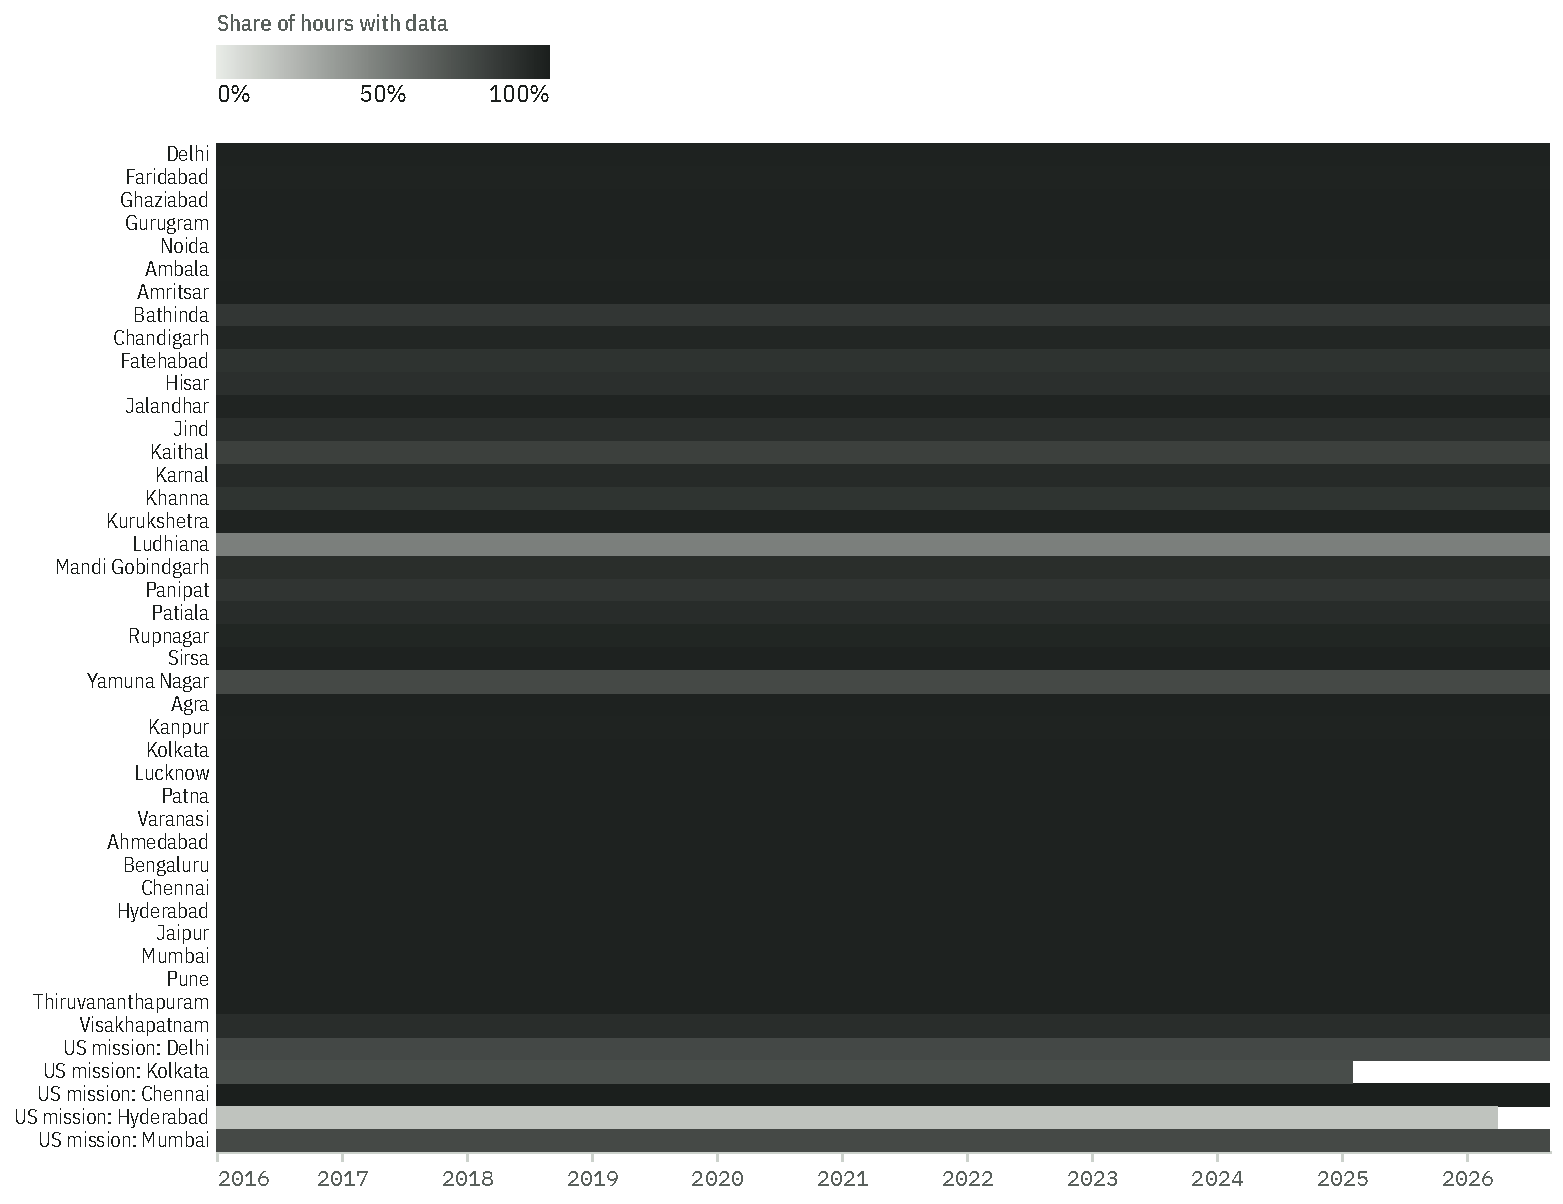
\includegraphics[width=1\linewidth,height=\textheight,keepaspectratio,alt={Share of hours with a valid PM2.5 reading, by city and month. CPCB-network data are missing from the OpenAQ archive from late 2022 to early 2025; the US mission monitors run almost without a break.}]{figures/fig02_coverage.pdf}
\caption{Share of hours with a valid PM2.5 reading, by city and month.
CPCB-network data are missing from the OpenAQ archive from late 2022 to
early 2025; the US mission monitors run almost without a break.}
\end{figure}

\subsection{Fire detections}\label{fire-detections}

Active-fire detections come from NASA FIRMS (\citeproc{ref-firms}{NASA
LANCE FIRMS 2026}): VIIRS on Suomi-NPP at 375 m
(\citeproc{ref-schroeder2014}{Schroeder et al. 2014}), which crosses
India at about 1:30 pm and 1:30 am local time, and MODIS
(\citeproc{ref-giglio2016}{Giglio et al. 2016}). We keep detections
classified as presumed vegetation fires, assign them to Punjab or
Haryana with state boundaries from geoBoundaries
(\citeproc{ref-geoboundaries}{{Runfola et al.} 2020}), and, as a
robustness check, drop 0.02° grid cells that light up in four or more
months outside the two crop-burning seasons (likely kilns, flares and
other fixed heat sources). VIIRS detections in Punjab and Haryana in
October--November track the official Punjab season counts closely in the
three years for which we have both.

\subsection{Weather}\label{weather}

Hourly temperature, humidity, precipitation, surface pressure, 10 m
wind, cloud cover, solar radiation and boundary-layer height for each
city come from the ERA5 reanalysis
(\citeproc{ref-hersbach2020}{{Hersbach et al.} 2020}) through the
Open-Meteo archive API (\citeproc{ref-zippenfenig2023}{Zippenfenig
2023}).

\section{Methods}\label{methods}

\subsection{Weather normalisation}\label{weather-normalisation}

For each site with at least 500 valid days we fit a LightGBM model
(\citeproc{ref-ke2017}{Ke et al. 2017}) of daily log PM2.5 on daily
weather summaries and calendar terms (a linear time trend, day of year
and day of week). Following Grange et al.
(\citeproc{ref-grange2018}{2018}), the weather-normalised value for each
day is the average of 200 predictions in which the weather columns are
replaced by draws from the site's whole record while the calendar terms
are kept. Predictions are back-transformed with Duan's smearing factor
(\citeproc{ref-duan1983}{Duan 1983}). Model skill comes from five-fold
cross-validation in which whole calendar years are held out together. To
compare winter with the monsoon, we compute the winter
(November--January) minus monsoon (July--September) gap in the observed
and the normalised series; the share of the observed gap that disappears
after normalisation is the share attributable to weather. For Delhi we
test for trend in the deseasonalised normalised monthly series with the
Theil--Sen estimator (\citeproc{ref-sen1968}{Sen 1968}) and Kendall's
test, and search for change points with PELT
(\citeproc{ref-killick2012}{Killick et al. 2012}).

\subsection{The Diwali baseline}\label{the-diwali-baseline}

For Delhi and four other cities we fit an hourly business-as-usual (BAU)
model of log PM2.5 on weather, rolling 6- and 24-hour summaries of wind,
boundary-layer height and rain, calendar terms and, for northern cities,
a wind-aware fire index (below) with lags of 0--3 days. Diwali windows
(three days either side) are never used for training, and every hour is
predicted out of fold, with whole ISO weeks held out together, so that
Diwali nights and ordinary nights are judged by the same standard. The
out-of-fold R² on log PM2.5 for ordinary hours is 0.75 for the US
Embassy and 0.78 for the CPCB network median.

The Diwali-night excess is the mean of observed minus BAU from 6 pm on
Diwali to 3 am the next morning. Because monitors often go missing
during the worst hours (Section 4.1), we fill missing hours inside the
window with the last valid reading. This is a rough lower bound, since
the monitors fail while concentrations are rising. Our main receptor is
the median across CPCB Delhi sites in hours with at least three
reporting, which is far less affected by single-monitor failures; the US
Embassy series is used as a cross-check. As a reference distribution we
apply the same calculation to every ordinary night between 1 October and
15 December, excluding the days around Dussehra, Chhath and Gurpurab.

For the fingerprint we compare 6 pm to midnight on Diwali with the same
hours on the five nights a week earlier at each CPCB Delhi site, for the
PM2.5/PM10 ratio, SO₂, CO and NO₂, using Wilcoxon signed-rank tests.

\subsection{Wind-aware fire index and
coupling}\label{wind-aware-fire-index-and-coupling}

For each day the fire index adds up VIIRS detections in Punjab and
Haryana, each weighted by max(0, cos θ), where θ is the angle between
the bearing from Delhi to the fire and the direction the wind is blowing
from, and by exp(−d/300 km), where d is the distance to Delhi. The
transport wind is the daily vector-mean 10 m wind at Delhi, Panipat,
Patiala and Ludhiana, along the Punjab--Delhi corridor. To find how long
smoke takes to arrive, we correlate the index at lags of 0--5 days with
the daily log-residual of a weather-only model of Delhi's PM2.5 (US
Embassy), after removing each season's mean. For coupling, we regress
the same residual on the index averaged over the strongest lags,
separately for each season (10 October--30 November, Diwali excluded),
with Newey--West standard errors (\citeproc{ref-newey1987}{Newey and
West 1987}).

\subsection{Ground test of a shift in burning
time}\label{ground-test-of-a-shift-in-burning-time}

If burning has moved into the evening, the evening share of PM2.5 at
monitors inside Punjab and Haryana should rise during the harvest. For
each site and season we compute the ratio of mean PM2.5 at 6
pm--midnight to that at 10 am--4 pm, during 15 October--30 November and
during 5--31 December of the same year, and compare the ratio of the two
between seasons.

\subsection{Pre-registered forecast}\label{pre-registered-forecast}

Before Diwali 2026 (8 November) we lock a forecast of the CPCB-network
Diwali-night excess for each possible firecracker regime: the mean of
past Diwalis under the same rules, with an 80\% prediction interval from
the variance pooled across regimes. The record is committed to the
public repository with its SHA-256 checksum.

\section{Results}\label{results}

\subsection{The monitor that goes
dark}\label{the-monitor-that-goes-dark}

At the US Embassy, 52\% of the hours between 10 pm and 3 am on Diwali
nights have no valid reading, against 4\% on ordinary autumn nights when
the monitor was running, about 13 times as often (Fig. 8). Gaps occurred
on 7 of 10 Diwali nights. They begin at 10 pm, one to three hours into
the evening rise, and often follow an hour or two in which the
instrument repeats its last reading. The CPCB network median, which
combines many monitors, lost 14\% of the same hours in the 7 Diwalis it
covers. The two records also disagree from year to year: their
Diwali-night excesses are uncorrelated (Pearson r = −0.11, 7 years). Any
Diwali estimate built from the Embassy record alone leaves out the peak.

\begin{figure}
\centering
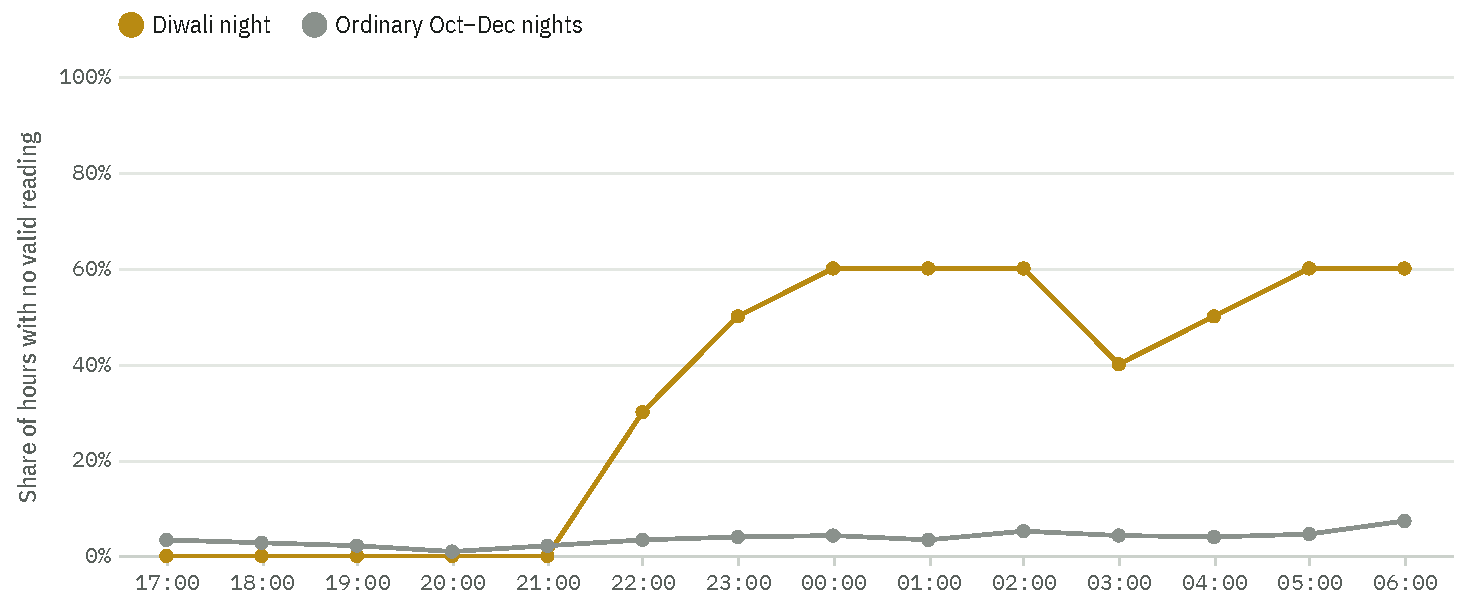
\includegraphics[width=1\linewidth,height=\textheight,keepaspectratio,alt={Share of hours with no valid reading at the US Embassy monitor, Diwali nights against ordinary autumn nights.}]{figures/fig08_censoring.pdf}
\caption{Share of hours with no valid reading at the US Embassy monitor,
Diwali nights against ordinary autumn nights.}
\end{figure}

\subsection{Weather and the winter
gap}\label{weather-and-the-winter-gap}

The daily weather models reach a median cross-validated R² of 0.52 on
log PM2.5 across 103 sites (interquartile range 0.28--0.68; 0.82 at the
US Embassy). We leave out of the comparison the 37 sites below R² = 0.4,
mostly short records in Punjab and Haryana where holding out whole years
leaves the model little to learn from. Across the remaining 66 sites in
23 cities, weather accounts for a median of 62\% of the
winter-minus-monsoon gap in Delhi-NCR (5 cities, range 61\%--68\%), 48\%
in Punjab and Haryana (7 cities, 39\%--62\%), 82\% in the rest of the
Gangetic Plain (6 cities) and 81\% outside the plain (5 cities; Fig. 4).
The burning belt stands out: where paddy residue is burned, weather
explains only about half of the winter rise, and in Delhi-NCR, downwind
of it, about three-fifths. Further east along the plain and in southern
and western cities, most of the seasonal swing is the monsoon washing
the air clean and the shallow winter boundary layer trapping what is
emitted all year. Removing weather shrinks the north--south difference
in winter PM2.5 from 45 to 33 µg/m³, so about 27\% of that difference is
weather and the rest is emissions.

Did the 2020 drop last? In Delhi, largely yes (Figs. 3 and 5). Over the
whole record the weather-normalised series at the US Embassy falls by
1.6\% a year (Theil--Sen), but the decline is not smooth: the only
change point PELT finds in the deseasonalised series is at 2020-01.
During the national lockdown, normalised PM2.5 was 14\% below its
2016--2019 level. From June 2020 to September 2026 it averaged 11\%
below that level (one-sided Mann--Whitney p \textless{} 0.001), and
within that later period it fell by only 0.5\% a year (95\% CI 0.0 to
0.9). The lower level that followed the lockdown held, but little
further progress followed it. Because the normalisation model includes a
smooth time trend, it may spread part of a sharp step over neighbouring
months; the step and the slope should be read together.

\begin{figure}
\centering
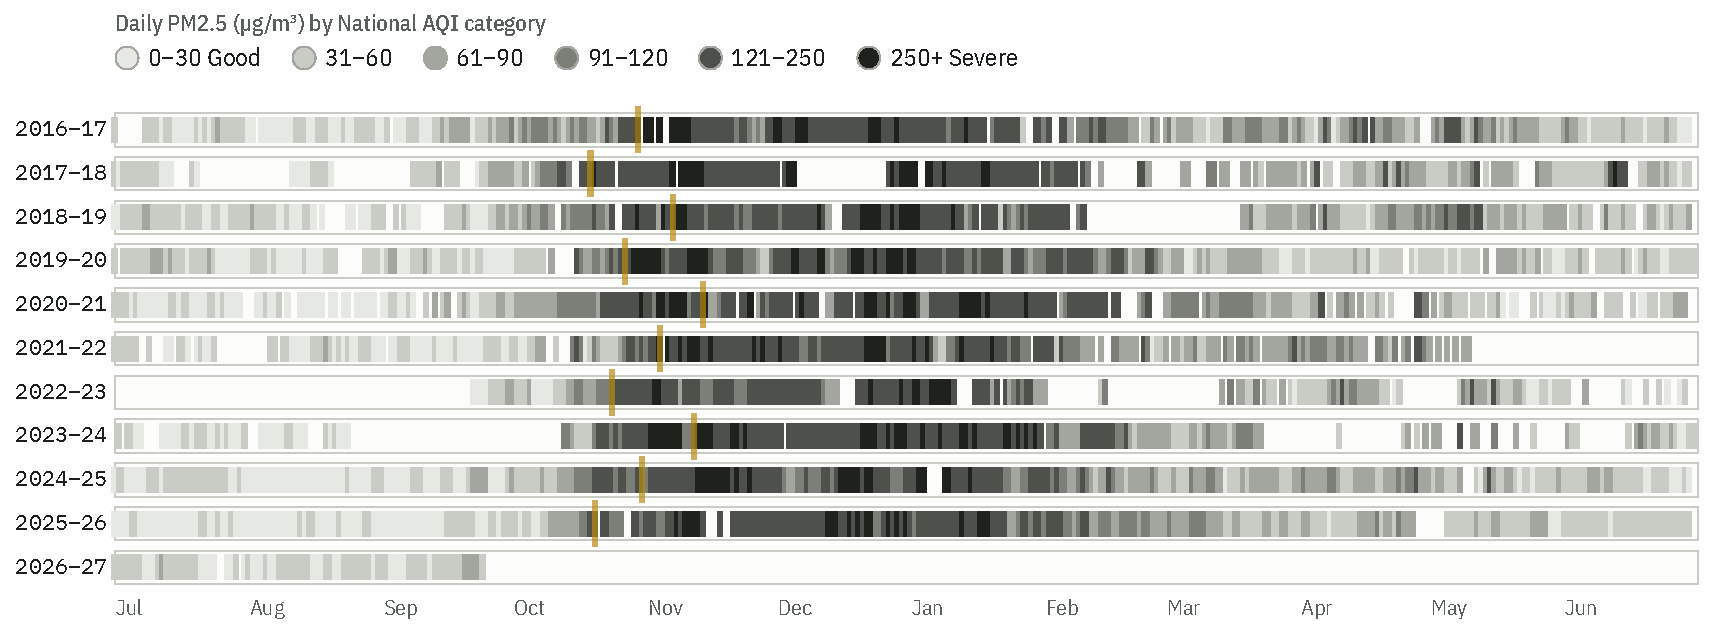
\includegraphics[width=1\linewidth,height=\textheight,keepaspectratio,alt={Daily mean PM2.5 at the US Embassy, one strip per season from July to June, shaded by India's National AQI category. Marigold ticks mark Diwali.}]{figures/fig03_tape.pdf}
\caption{Daily mean PM2.5 at the US Embassy, one strip per season from
July to June, shaded by India's National AQI category. Marigold ticks
mark Diwali.}
\end{figure}

\begin{figure}
\centering
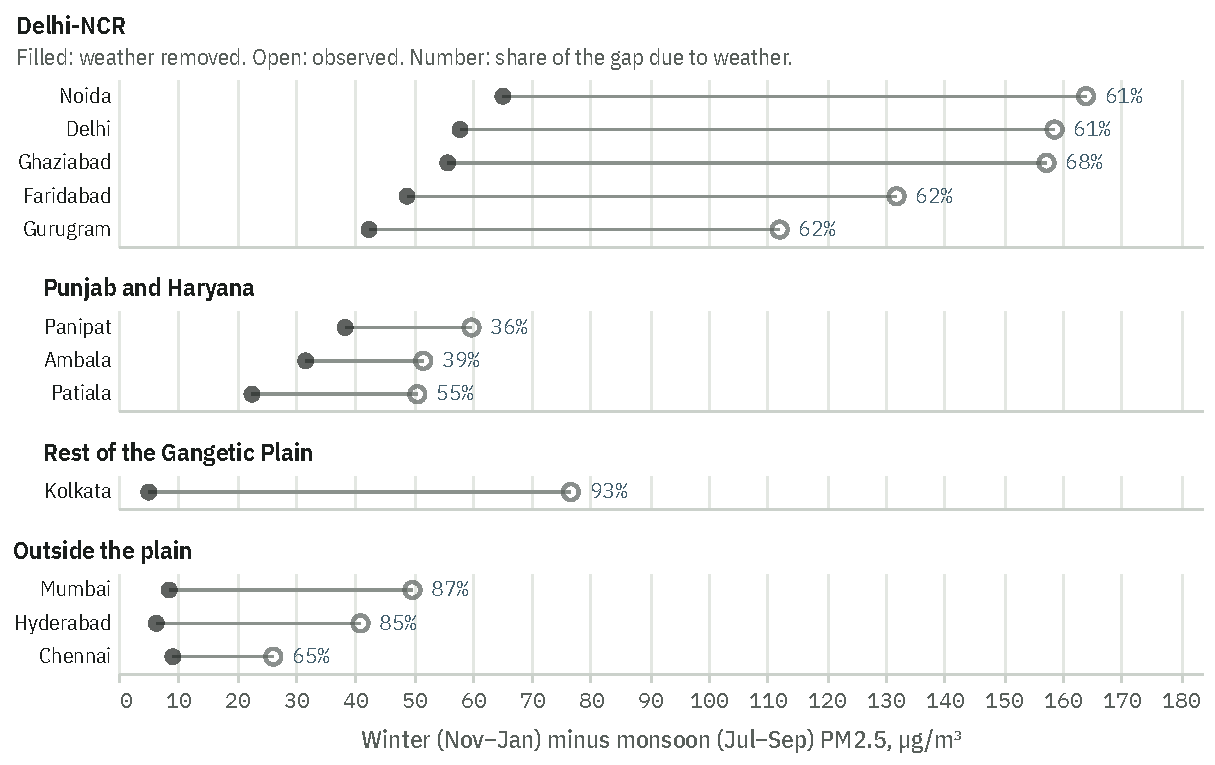
\includegraphics[width=1\linewidth,height=\textheight,keepaspectratio,alt={Winter (Nov--Jan) minus monsoon (Jul--Sep) PM2.5 by city, as observed (open circle) and after removing weather (filled). The number is the share of the gap that weather accounts for.}]{figures/fig04_gap.pdf}
\caption{Winter (Nov--Jan) minus monsoon (Jul--Sep) PM2.5 by city, as
observed (open circle) and after removing weather (filled). The number
is the share of the gap that weather accounts for.}
\end{figure}

\begin{figure}
\centering
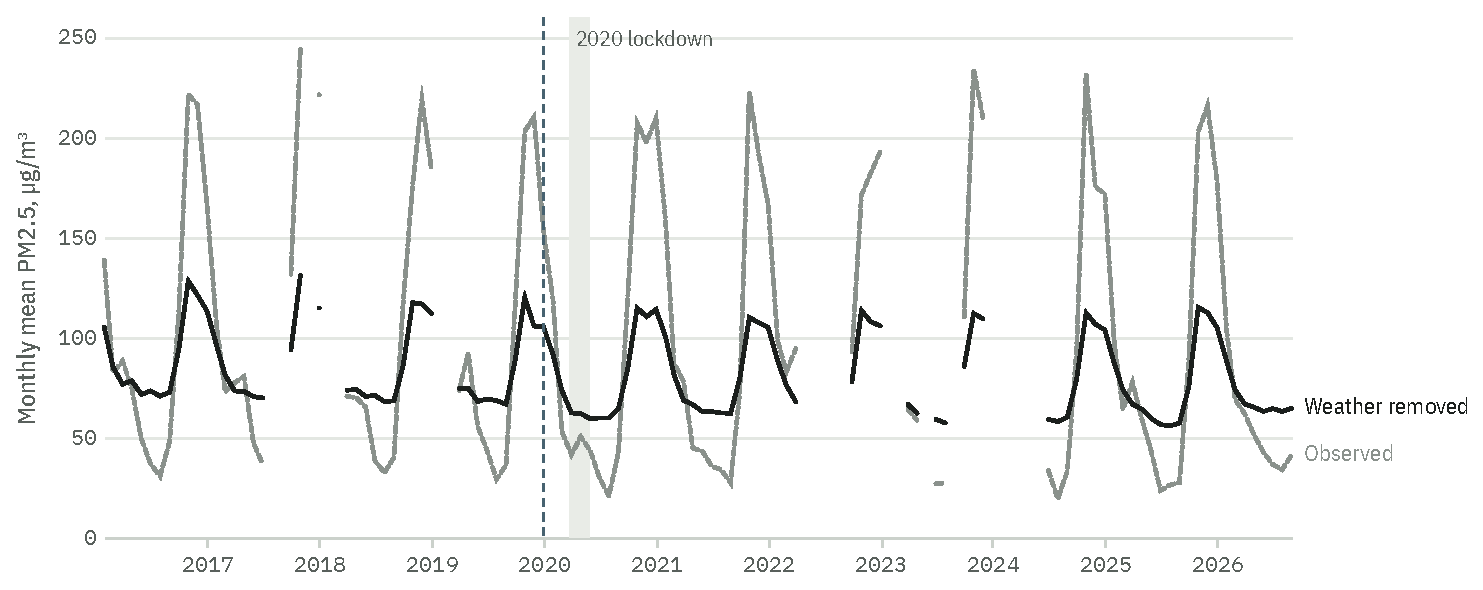
\includegraphics[width=1\linewidth,height=\textheight,keepaspectratio,alt={Monthly PM2.5 at the US Embassy, observed and weather-normalised. The dashed line marks the change point found in the deseasonalised normalised series; the shaded band is the 2020 national lockdown.}]{figures/fig05_trend.pdf}
\caption{Monthly PM2.5 at the US Embassy, observed and
weather-normalised. The dashed line marks the change point found in the
deseasonalised normalised series; the shaded band is the 2020 national
lockdown.}
\end{figure}

\subsection{Diwali}\label{diwali}

In every year with data, Diwali night rises far above the
weather-and-fire baseline (Fig. 6). In the CPCB network median the
excess ranged from 127 to 392 µg/m³ (mean 289), against a 99th
percentile of 193 µg/m³ across 211 ordinary nights; 6 of 7 Diwali nights
exceeded it (Fig. 7).

The firecracker rules made no visible difference. The mean excess was
192 µg/m³ in the two years without a bursting restriction (2016, 2017),
303 µg/m³ in green-cracker years (2018, 2019, 2025) and 366 µg/m³ in the
full-ban years the network covers (2020, 2021) (Kruskal--Wallis p =
0.18). The samples are small and the archive gap removes three full-ban
Diwalis, so this is descriptive, but nothing in the record suggests the
bans shrank the spike. The smallest excess (128 µg/m³) came in 2017,
when the Supreme Court suspended sales in Delhi-NCR about ten days
before an early Diwali (9 and 19 October). The two largest came in 2021,
under a full ban (392), and 2025, the first year green crackers were
allowed again (386), which also had the fewest farm fires of the decade.

The farm-fire term matters little on Diwali night. Including it in the
baseline changed the US Embassy Diwali excess by a median of −5 µg/m³,
and with or without it the excess is unrelated to the fire exposure on
Diwali night (Spearman ρ = −0.31 and −0.22, n = 10, neither
significant). The festival's excess is local; it is not farm smoke being
misattributed.

The Diwali evening carries a firework fingerprint at CPCB Delhi sites
(Fig. 10). Against the same hours a week earlier, the PM2.5/PM10 ratio
rose in 96\% of 47 site-years (median 0.41 → 0.69, Wilcoxon p
\textless{} 0.001), so the extra particles are fine ones, and SO₂,
released by the sulphur in fireworks, rose in 70\% (median +37\%, p
\textless{} 0.001). The traffic gases moved the other way: NO₂ changed
by a median of −8\% and CO by −11\%, consistent with fewer vehicles on
the road on Diwali evening. A rise in fine particles and SO₂ without a
rise in NO₂ and CO points to fireworks rather than traffic or a general
build-up.

The timing follows local custom (Fig. 9). In Delhi the median excess
peaks around midnight and stays high until morning. In Mumbai and
Hyderabad it peaks between 8 and 11 pm on Diwali. In Chennai the largest
peak comes on the evening before Diwali as dated in Delhi, consistent
with Deepavali being celebrated on Naraka Chaturdashi in Tamil Nadu;
Kolkata, with few years of data, shows peaks on both evenings.

\begin{figure}
\centering
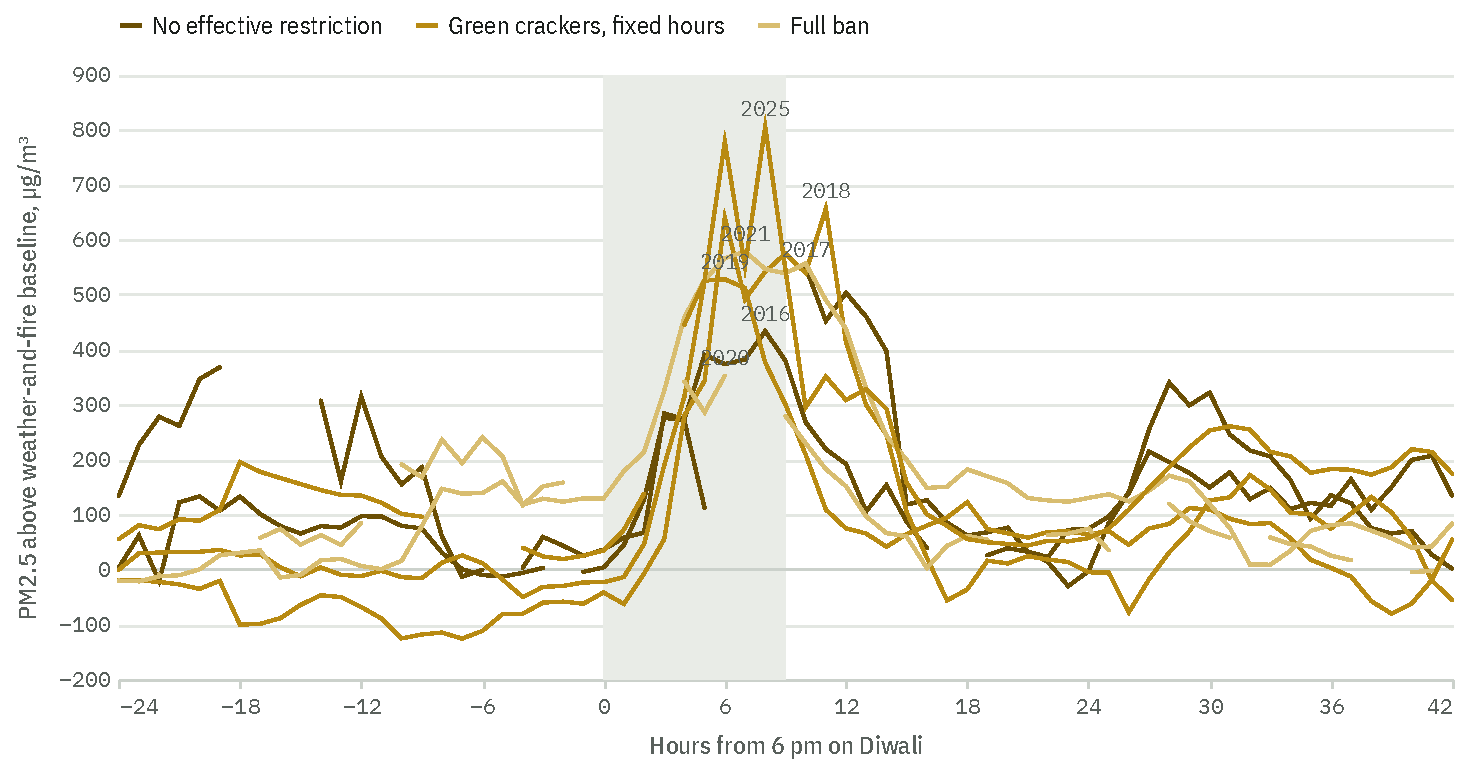
\includegraphics[width=1\linewidth,height=\textheight,keepaspectratio,alt={Hourly PM2.5 above the business-as-usual baseline (weather, calendar and wind-aware fire index) around Diwali night, CPCB Delhi network median, one line per year coloured by the firecracker rules. Shading marks 6 pm--3 am.}]{figures/fig06_event.pdf}
\caption{Hourly PM2.5 above the business-as-usual baseline (weather,
calendar and wind-aware fire index) around Diwali night, CPCB Delhi
network median, one line per year coloured by the firecracker rules.
Shading marks 6 pm--3 am.}
\end{figure}

\begin{figure}
\centering
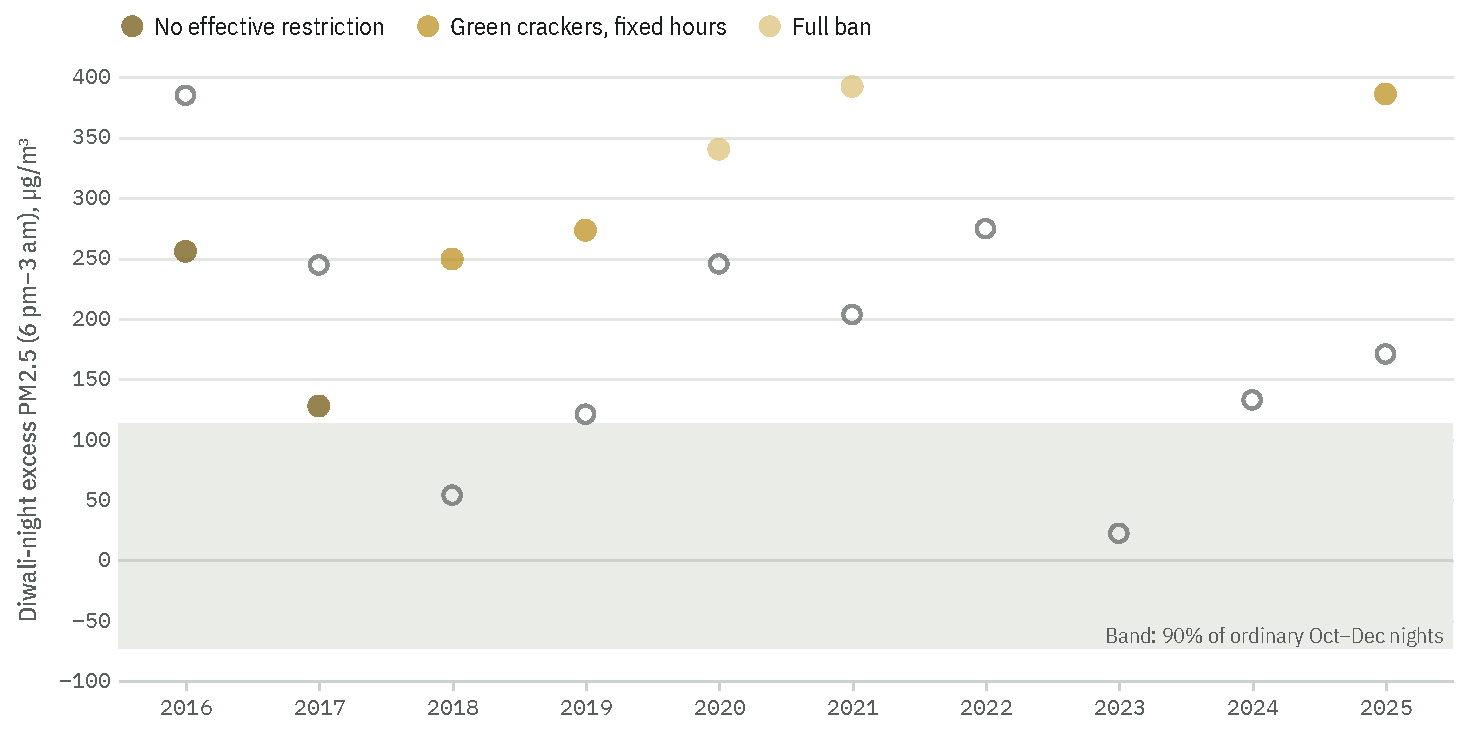
\includegraphics[width=1\linewidth,height=\textheight,keepaspectratio,alt={Diwali-night excess PM2.5 (6 pm--3 am, above the weather-and-fire baseline) by year. Filled points: CPCB network median, coloured by the firecracker rules. Open circles: US Embassy, with missing hours carried forward. The band covers 90\% of ordinary October--December nights in the network median.}]{figures/fig07_nights.pdf}
\caption{Diwali-night excess PM2.5 (6 pm--3 am, above the
weather-and-fire baseline) by year. Filled points: CPCB network median,
coloured by the firecracker rules. Open circles: US Embassy, with
missing hours carried forward. The band covers 90\% of ordinary
October--December nights in the network median.}
\end{figure}

\begin{figure}
\centering
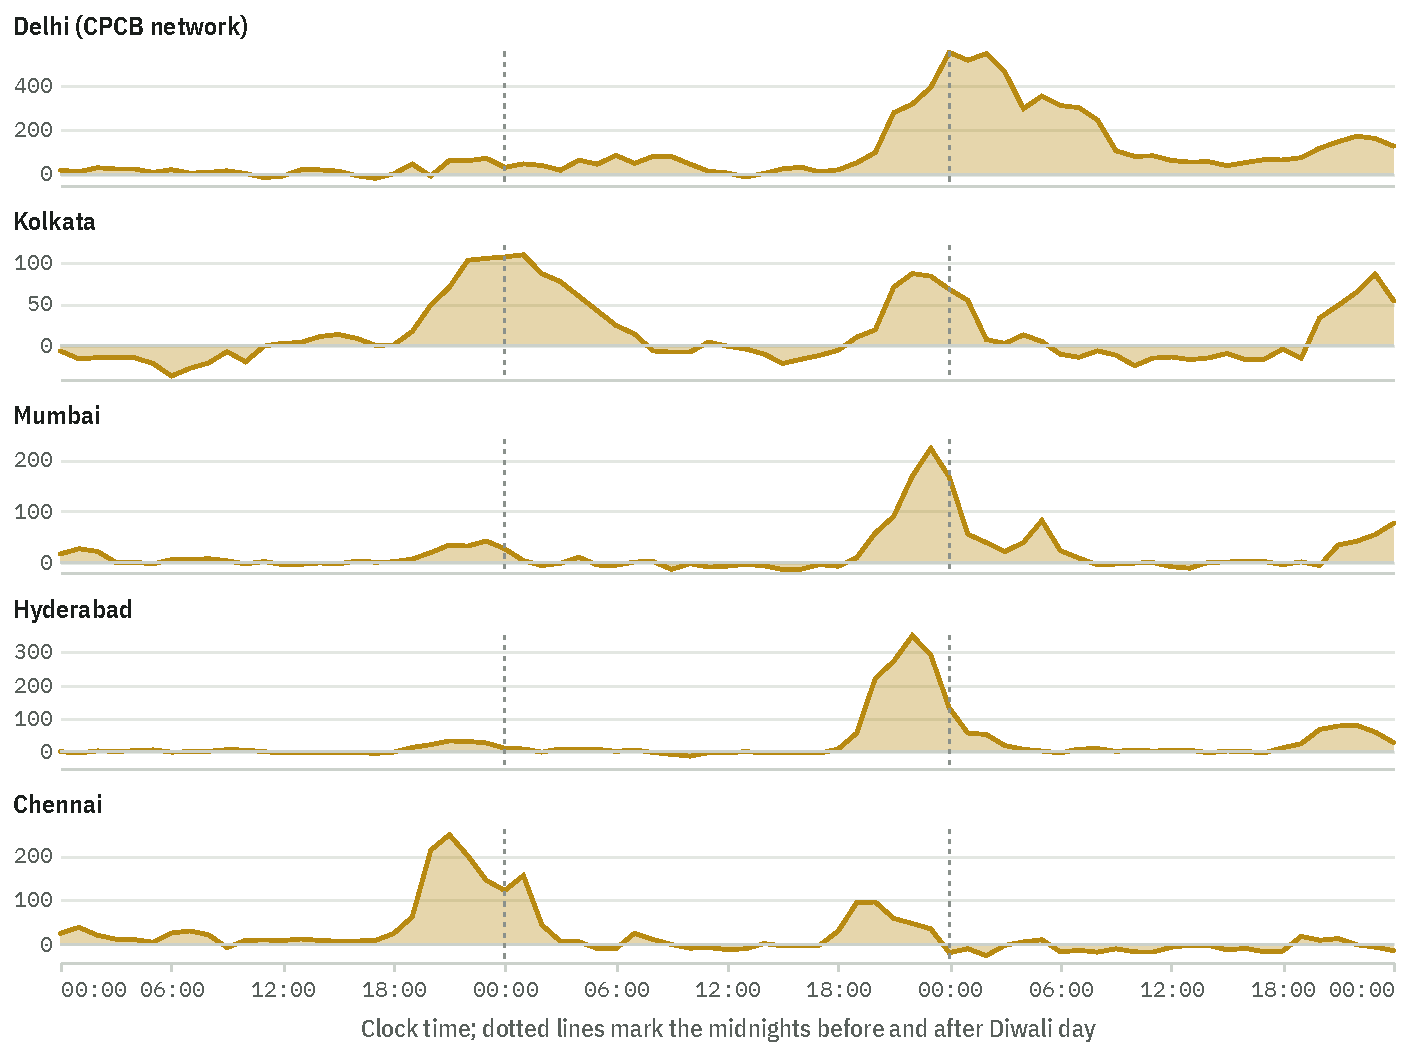
\includegraphics[width=1\linewidth,height=\textheight,keepaspectratio,alt={Median hourly excess PM2.5 above the baseline around Diwali in five cities (Delhi: CPCB network median; others: US mission monitors). Dotted lines mark the midnights before and after Diwali day as dated in Delhi.}]{figures/fig09_cities.pdf}
\caption{Median hourly excess PM2.5 above the baseline around Diwali in
five cities (Delhi: CPCB network median; others: US mission monitors).
Dotted lines mark the midnights before and after Diwali day as dated in
Delhi.}
\end{figure}

\begin{figure}
\centering
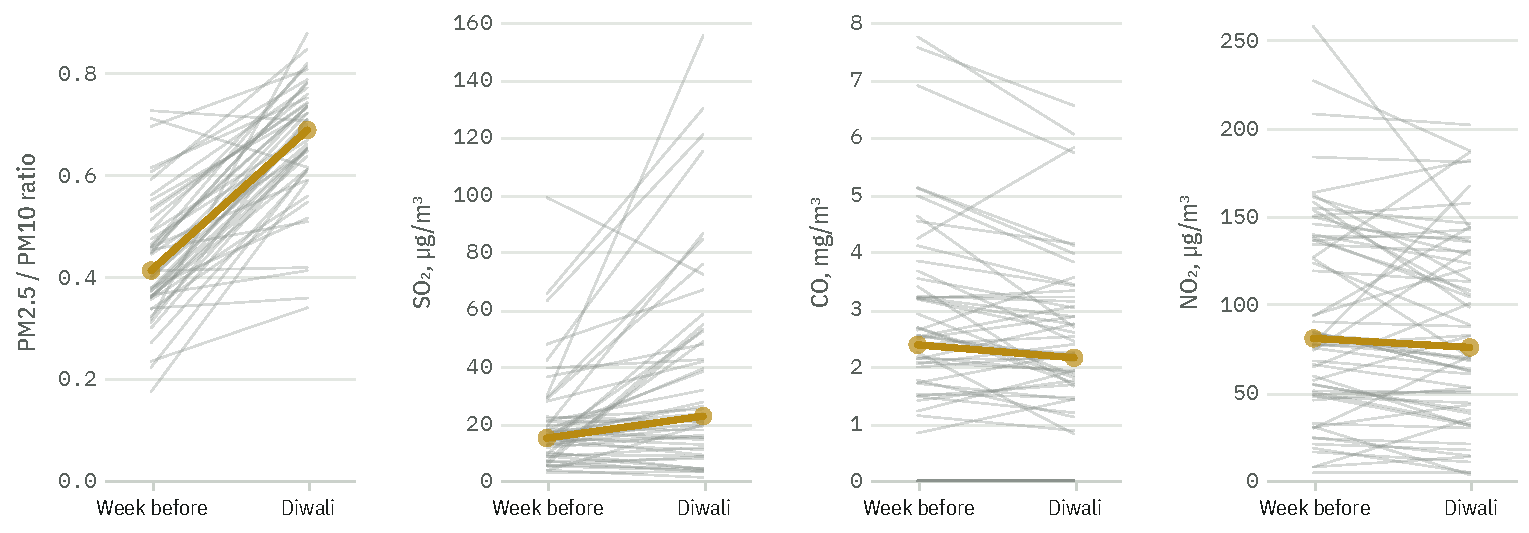
\includegraphics[width=1\linewidth,height=\textheight,keepaspectratio,alt={Diwali evening (6 pm--midnight) against the same hours on the five nights a week earlier, at CPCB Delhi sites. Thin lines are site-years; the thick line joins the medians.}]{figures/fig10_fingerprint.pdf}
\caption{Diwali evening (6 pm--midnight) against the same hours on the
five nights a week earlier, at CPCB Delhi sites. Thin lines are
site-years; the thick line joins the medians.}
\end{figure}

\subsection{The fire-count paradox}\label{the-fire-count-paradox}

VIIRS detections in Punjab and Haryana during October--November peaked
at 100,736 in 2016 and fell to 5,121 in 2025, 94\% below 2021 (Fig. 11).
The night pass tells a different story. Before 2024 the 1:30 am pass
caught 0.2\% of detections on average; in 2024 it caught 3.6\% and in
2025 4.7\%. In Punjab, night-pass detections reached 91 in 2024 and 77
in 2025, against at most 43 in any season from 2016 to 2023, even though
daytime detections fell by more than 90\%. The rise survives removal of
fixed heat sources. A satellite that only looks twice a day cannot show
when fires start, but more fires still burning at 1:30 am is what a
shift of ignition into the evening would produce, and it agrees with
geostationary evidence reported elsewhere
(\citeproc{ref-iforest2025}{{iFOREST} 2025};
\citeproc{ref-nasaeo2025}{NASA Earth Observatory 2025}).

Delhi's weather-adjusted PM2.5 responds to the fire index over one to
four days rather than on a single day: Spearman ρ is 0.10 on the same
day and between 0.16 and 0.17 at lags of one to four days. Per unit of
the index, the response was small and fairly stable in 2016--2021 (mean
2.2\% per 100 index units) and about ten times larger in 2025 (25\%,
95\% CI 0 to 55\%; Fig. 12). The 2025 interval is wide and only just
excludes zero, and 2024 is too uncertain to read, so this is suggestive
rather than conclusive. It is, however, what an undercount would
produce: if each detected fire stands for more burning than before, each
detection goes with more smoke. This offers a second explanation for the
weak coupling between counts and Delhi's air reported by {Mangaraj et
al.} (\citeproc{ref-mangaraj2025}{2025}), alongside the local controls
they discuss. To make the estimate robust to how the data are split, the
residuals behind it average predictions over five random cross-fitting
splits.

The ground test at 31 site-seasons in Punjab and Haryana does not show
the shift (Fig. 13): the harvest-to-December evening ratio had a median
of 1.19 before 2022 and 1.12 in 2025 (one-sided Mann--Whitney p = 0.95).
With the archive gap, the later period rests on few seasons, and 2025
had so little burning that a change in its timing would barely move
urban monitors.

\begin{figure}
\centering
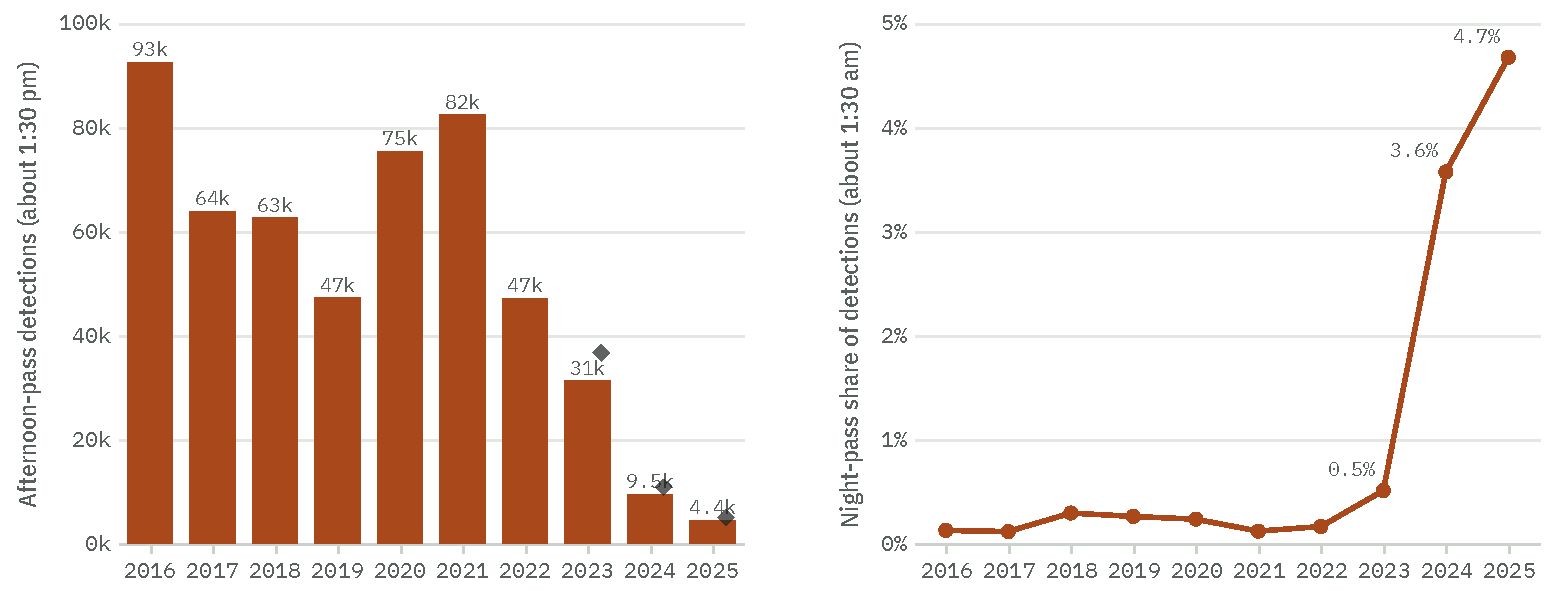
\includegraphics[width=1\linewidth,height=\textheight,keepaspectratio,alt={VIIRS S-NPP fire detections in Punjab and Haryana, October--November, split by overpass, after removing fixed heat sources. Diamonds mark official Punjab season counts.}]{figures/fig11_fires.pdf}
\caption{VIIRS S-NPP fire detections in Punjab and Haryana,
October--November, split by overpass, after removing fixed heat sources.
Diamonds mark official Punjab season counts.}
\end{figure}

\begin{figure}
\centering
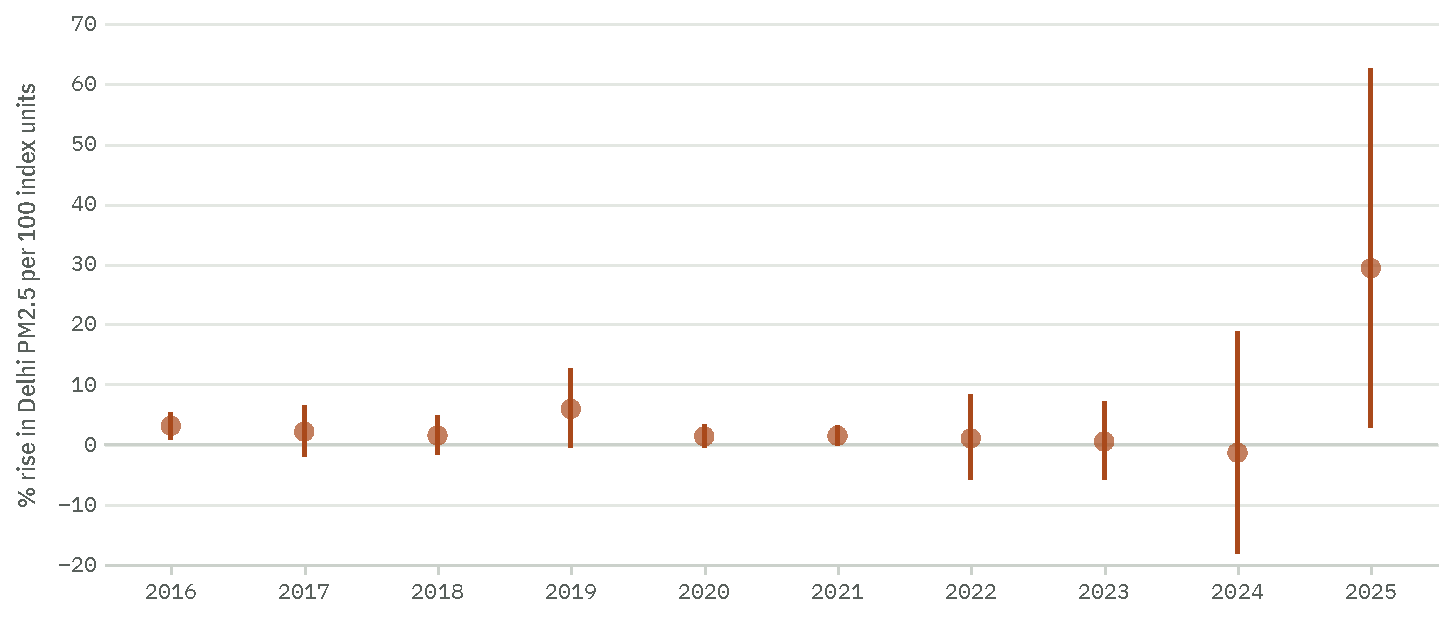
\includegraphics[width=1\linewidth,height=\textheight,keepaspectratio,alt={Percent change in Delhi's weather-adjusted PM2.5 per 100 units of the wind-aware fire index, by season, with 95\% confidence intervals (HAC standard errors).}]{figures/fig12_coupling.pdf}
\caption{Percent change in Delhi's weather-adjusted PM2.5 per 100 units
of the wind-aware fire index, by season, with 95\% confidence intervals
(HAC standard errors).}
\end{figure}

\begin{figure}
\centering
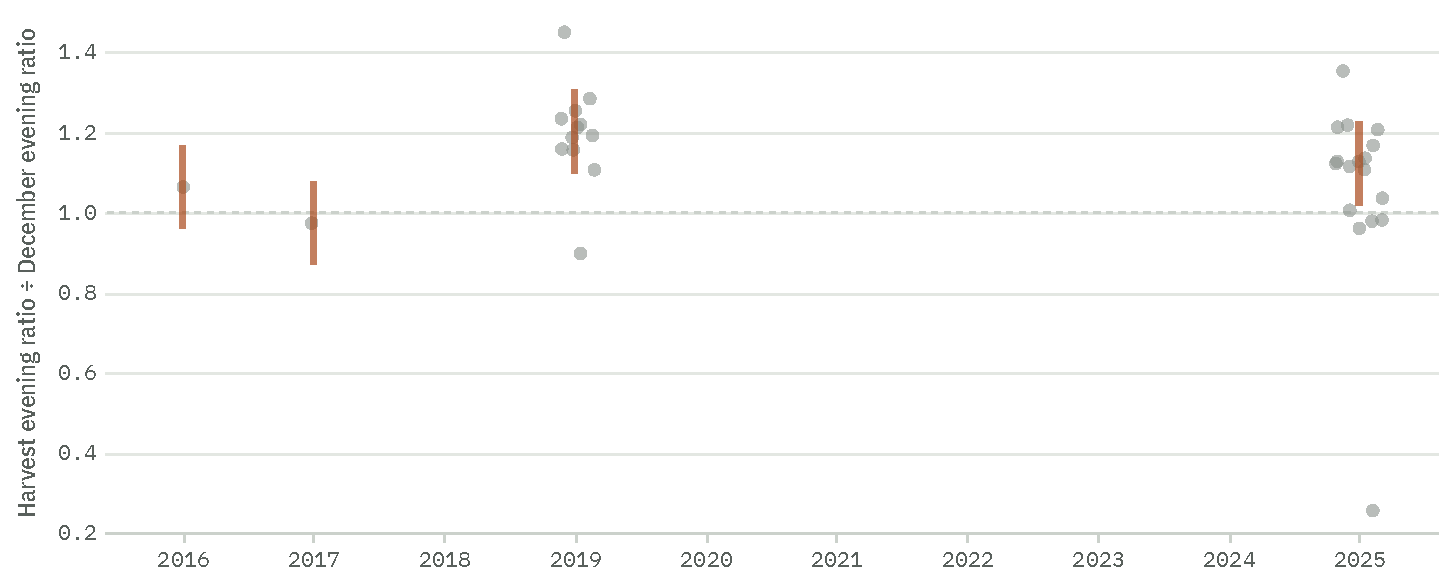
\includegraphics[width=1\linewidth,height=\textheight,keepaspectratio,alt={Evening-to-midday PM2.5 ratio in the harvest window divided by the same ratio in December, per monitor and season. Ticks mark the median. Values above 1 mean the evening share rises at harvest.}]{figures/fig13_evening.pdf}
\caption{Evening-to-midday PM2.5 ratio in the harvest window divided by
the same ratio in December, per monitor and season. Ticks mark the
median. Values above 1 mean the evening share rises at harvest.}
\end{figure}

\subsection{A forecast for Diwali
2026}\label{a-forecast-for-diwali-2026}

Table 1 gives the locked forecast. The record was committed on
2026-10-12 with SHA-256 checksum \texttt{0b5f3a06349b1dd1…}.

\begin{longtable}[]{@{}
  >{\raggedright\arraybackslash}p{(\linewidth - 6\tabcolsep) * \real{0.2143}}
  >{\raggedleft\arraybackslash}p{(\linewidth - 6\tabcolsep) * \real{0.2857}}
  >{\raggedleft\arraybackslash}p{(\linewidth - 6\tabcolsep) * \real{0.2857}}
  >{\raggedright\arraybackslash}p{(\linewidth - 6\tabcolsep) * \real{0.2143}}@{}}
\caption{Locked forecast of the Diwali-night excess in the CPCB Delhi
network median, 8 November 2026.}\tabularnewline
\toprule\noalign{}
\begin{minipage}[b]{\linewidth}\raggedright
Firecracker rules in 2026
\end{minipage} & \begin{minipage}[b]{\linewidth}\raggedleft
Forecast excess (µg/m³)
\end{minipage} & \begin{minipage}[b]{\linewidth}\raggedleft
80\% interval
\end{minipage} & \begin{minipage}[b]{\linewidth}\raggedright
Past Diwalis used
\end{minipage} \\
\midrule\noalign{}
\endfirsthead
\toprule\noalign{}
\begin{minipage}[b]{\linewidth}\raggedright
Firecracker rules in 2026
\end{minipage} & \begin{minipage}[b]{\linewidth}\raggedleft
Forecast excess (µg/m³)
\end{minipage} & \begin{minipage}[b]{\linewidth}\raggedleft
80\% interval
\end{minipage} & \begin{minipage}[b]{\linewidth}\raggedright
Past Diwalis used
\end{minipage} \\
\midrule\noalign{}
\endhead
\bottomrule\noalign{}
\endlastfoot
Full ban & 366 & 233 to 499 & 2020, 2021 \\
Green crackers, fixed hours & 303 & 177 to 428 & 2018, 2019, 2025 \\
No effective restriction & 192 & 58 to 325 & 2016, 2017 \\
\end{longtable}

\begin{figure}
\centering
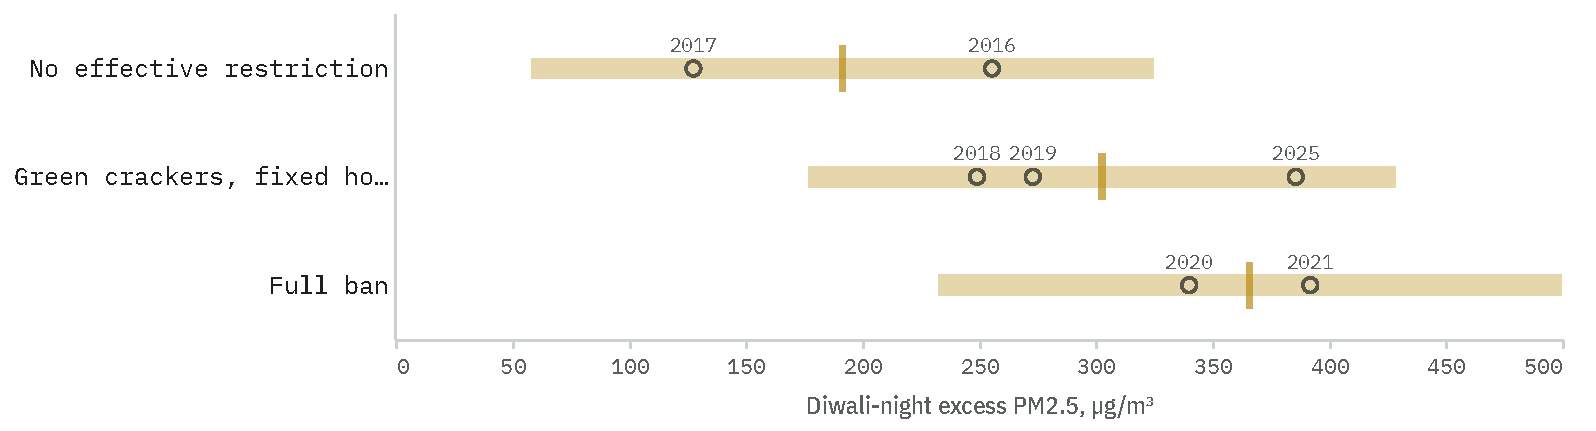
\includegraphics[width=1\linewidth,height=\textheight,keepaspectratio,alt={Forecast Diwali-night excess PM2.5 for 8 November 2026 under each possible firecracker regime, with 80\% prediction intervals. Open circles are past Diwalis under the same rules.}]{figures/fig14_forecast.pdf}
\caption{Forecast Diwali-night excess PM2.5 for 8 November 2026 under
each possible firecracker regime, with 80\% prediction intervals. Open
circles are past Diwalis under the same rules.}
\end{figure}

\section{Discussion}\label{discussion}

\textbf{Fire counts are losing their meaning as a target.} Official
progress on stubble burning is reported in active-fire counts. Our
results add one clear and one suggestive line of evidence that these
counts now understate burning: the night pass of the same satellite sees
a growing share of fires, and in 2025 each detected fire went with a
larger rise in Delhi's PM2.5. Reported declines of 80--90\% in counts
should not be read as declines of the same size in burning or in its
effect on Delhi. Burnt-area mapping and geostationary sensors, which do
not depend on a single overpass time, are better suited to tracking
progress.

\textbf{The firecracker bans did not shrink Diwali night.} Across the 7
Diwalis the network covers, the weather- and fire-adjusted excess was no
lower under a full ban than with green crackers or no bursting
restriction. This matches the Supreme Court's own observation in 2025
that air quality differed little between green-cracker and full-ban
years (\citeproc{ref-dh2025}{Deccan Herald 2025}). It suggests the bans
were not effectively enforced, though our data cannot show why. The one
low year, 2017, followed a sales suspension ordered about ten days
ahead, which may be worth studying as a design that limits supply rather
than use.

\textbf{Monitoring fails when it matters most.} The monitor most widely
used as Delhi's reference stops reporting during the hours of highest
concentration on Diwali night. Studies and dashboards that average
whatever hours survive will understate the festival. Reporting the
number of missing hours alongside any Diwali figure, and using the
network median rather than a single monitor, are simple remedies.

\section{Limitations}\label{limitations}

The CPCB archive gap from late 2022 to early 2025 removes three Diwalis
and three burning seasons from the network record; for these years we
rely on the US Embassy monitor, which is censored on Diwali night. The
regime comparison rests on two or three Diwalis per regime and is
descriptive. The fire-coupling estimate for 2025 rests on one season
with very few detected fires. The fire index uses surface winds, while
smoke travels at higher levels. Rural Punjab has few monitors, so the
ground test uses urban ones, where local sources dominate the evening.
Weather normalisation removes the effect of weather on average; it
cannot remove every interaction between weather and emissions. Diwali
dates and firecracker rules are compiled from secondary reports and
should be checked against the original orders.

\section{Conclusions}\label{conclusions}

Separating weather, farm smoke and fireworks with public data and open
code is feasible, and the separation changes the story. Diwali adds a
large, consistent excess that the firecracker bans have not visibly
reduced. The fall in fire counts very likely overstates the fall in
burning. And the reference monitor goes dark at the peak. We will score
our Diwali 2026 forecast in public after the festival.

\section{Data and code availability}\label{data-and-code-availability}

All code, derived tables, figures and the locked forecast are at
https://github.com/krishnav1412/eleven-winters. The companion website,
including a city explorer for the 103 sites with weather-normalised
series, is at https://krishnav1412.github.io/eleven-winters/. Raw data
are public: OpenAQ, NASA FIRMS and ERA5 via Open-Meteo. One command
(\texttt{ew\ all}) rebuilds every result from the raw data.

\section*{References}\label{references}
\addcontentsline{toc}{section}{References}

\protect\phantomsection\label{refs}
\begin{CSLReferences}{1}{1}
\bibitem[\citeproctext]{ref-biswal2025}
Biswal, Akash, Masayuki Takigawa, Poonam Mangaraj, et al. 2025.
{``Emission Time and Amount of Crop Residue Burning Play Critical Role
on {PM2.5} Variability During {October--November} in Northwestern
{India} During 2022--2024.''} \emph{Environmental Science: Atmospheres}
5: 1211--29. \url{https://doi.org/10.1039/D5EA00052A}.

\bibitem[\citeproctext]{ref-dh2025}
Deccan Herald. 2025. \emph{Diwali 2025: {SC} Allows Green Crackers in
{Delhi-NCR}; Rules, Timings and Pollution Concerns}.
\href{https://www.deccanherald.com/india/diwali-2025-sc-allows-green-crackers-in-delhi-ncr-rules-timings-pollution-concerns-3765583}{Https://www.deccanherald.com/india/diwali-2025-sc-allows-green-crackers-in-delhi-ncr-rules-timings-pollution-concerns-3765583}.

\bibitem[\citeproctext]{ref-duan1983}
Duan, Naihua. 1983. {``Smearing Estimate: A Nonparametric
Retransformation Method.''} \emph{Journal of the American Statistical
Association} 78 (383): 605--10.
\url{https://doi.org/10.1080/01621459.1983.10478017}.

\bibitem[\citeproctext]{ref-ghei2018}
Ghei, Deepshikha, and Renuka Sane. 2018. {``Estimates of Air Pollution
in {Delhi} from the Burning of Firecrackers During the Festival of
{Diwali}.''} \emph{PLoS ONE} 13 (8): e0200371.
\url{https://doi.org/10.1371/journal.pone.0200371}.

\bibitem[\citeproctext]{ref-giglio2016}
Giglio, Louis, Wilfrid Schroeder, and Christopher O. Justice. 2016.
{``The Collection 6 {MODIS} Active Fire Detection Algorithm and Fire
Products.''} \emph{Remote Sensing of Environment} 178: 31--41.
\url{https://doi.org/10.1016/j.rse.2016.02.054}.

\bibitem[\citeproctext]{ref-grange2018}
Grange, Stuart K., David C. Carslaw, Alastair C. Lewis, Eirini Boleti,
and Christoph Hueglin. 2018. {``Random Forest Meteorological
Normalisation Models for {Swiss} {PM10} Trend Analysis.''}
\emph{Atmospheric Chemistry and Physics} 18: 6223--39.
\url{https://doi.org/10.5194/acp-18-6223-2018}.

\bibitem[\citeproctext]{ref-hei_ncap}
Health Effects Institute. 2025. \emph{Assessing {India}'s {National
Clean Air Programme}: Webinar Slides}.
\href{https://www.healtheffects.org/sites/default/files/india-ncap-assessment-webinar.pdf}{Https://www.healtheffects.org/sites/default/files/india-ncap-assessment-webinar.pdf}.

\bibitem[\citeproctext]{ref-hersbach2020}
{Hersbach, Hans, Bill Bell, Paul Berrisford, et al.} 2020. {``The {ERA5}
Global Reanalysis.''} \emph{Quarterly Journal of the Royal
Meteorological Society} 146 (730): 1999--2049.
\url{https://doi.org/10.1002/qj.3803}.

\bibitem[\citeproctext]{ref-iforest2025}
{iFOREST}. 2025. \emph{Stubble Burning Status Report 2025}. iFOREST.

\bibitem[\citeproctext]{ref-ke2017}
Ke, Guolin, Qi Meng, Thomas Finley, et al. 2017. {``{LightGBM}: A Highly
Efficient Gradient Boosting Decision Tree.''} \emph{Advances in Neural
Information Processing Systems} 30.

\bibitem[\citeproctext]{ref-killick2012}
Killick, Rebecca, Paul Fearnhead, and Idris A. Eckley. 2012. {``Optimal
Detection of Changepoints with a Linear Computational Cost.''}
\emph{Journal of the American Statistical Association} 107 (500):
1590--98. \url{https://doi.org/10.1080/01621459.2012.737745}.

\bibitem[\citeproctext]{ref-mangaraj2025}
{Mangaraj, Poonam, Yutaka Matsumi, Tomoki Nakayama, et al.} 2025.
{``Weak Coupling of Observed Surface {PM2.5} in {Delhi-NCR} with Rice
Crop Residue Burning in {Punjab} and {Haryana}.''} \emph{Npj Climate and
Atmospheric Science} 8.
\url{https://doi.org/10.1038/s41612-025-00901-8}.

\bibitem[\citeproctext]{ref-nasaeo2025}
NASA Earth Observatory. 2025. \emph{New Timing for Stubble Burning in
{India}}.
\href{https://science.nasa.gov/earth/earth-observatory/new-timing-for-stubble-burning-in-india}{Https://science.nasa.gov/earth/earth-observatory/new-timing-for-stubble-burning-in-india}.

\bibitem[\citeproctext]{ref-firms}
NASA LANCE FIRMS. 2026. \emph{Fire Information for Resource Management
System: Country Yearly Active Fire Data ({MODIS} {C6.1}, {VIIRS} {S-NPP}
375 m)}.
\href{https://firms.modaps.eosdis.nasa.gov/country/}{Https://firms.modaps.eosdis.nasa.gov/country/}.

\bibitem[\citeproctext]{ref-newey1987}
Newey, Whitney K., and Kenneth D. West. 1987. {``A Simple, Positive
Semi-Definite, Heteroskedasticity and Autocorrelation Consistent
Covariance Matrix.''} \emph{Econometrica} 55 (3): 703--8.
\url{https://doi.org/10.2307/1913610}.

\bibitem[\citeproctext]{ref-openaq}
OpenAQ. 2026. \emph{{OpenAQ} Open Data Archive on {AWS}}.
\href{https://registry.opendata.aws/openaq/}{Https://registry.opendata.aws/openaq/}.

\bibitem[\citeproctext]{ref-geoboundaries}
{Runfola, Daniel et al.} 2020. {``{geoBoundaries}: A Global Database of
Political Administrative Boundaries.''} In \emph{PLoS ONE}, No. 4, vol.
15. \url{https://doi.org/10.1371/journal.pone.0231866}.

\bibitem[\citeproctext]{ref-schroeder2014}
Schroeder, Wilfrid, Patricia Oliva, Louis Giglio, and Ivan A. Csiszar.
2014. {``The New {VIIRS} 375 m Active Fire Detection Data Product:
Algorithm Description and Initial Assessment.''} \emph{Remote Sensing of
Environment} 143: 85--96.
\url{https://doi.org/10.1016/j.rse.2013.12.008}.

\bibitem[\citeproctext]{ref-sen1968}
Sen, Pranab Kumar. 1968. {``Estimates of the Regression Coefficient
Based on {Kendall}'s Tau.''} \emph{Journal of the American Statistical
Association} 63 (324): 1379--89.
\url{https://doi.org/10.1080/01621459.1968.10480934}.

\bibitem[\citeproctext]{ref-verma2025}
Verma, Shubhi, Mohammad Rafiuddin, Uday Suryanarayanan, Shikhar Tiwari,
and Rishikesh Puravankara. 2025. {``Investigating the Impact of
Meteorology and Emissions on {PM2.5} and {PM10} in {Delhi} Using Machine
Learning.''} \emph{EGUsphere {[}Preprint{]}}, ahead of print.
\url{https://doi.org/10.5194/egusphere-2025-2300}.

\bibitem[\citeproctext]{ref-zippenfenig2023}
Zippenfenig, Patrick. 2023. \emph{{Open-Meteo.com} Weather {API}}.
Zenodo. \url{https://doi.org/10.5281/zenodo.7970649}.

\end{CSLReferences}

\end{document}
